%%%%%%%%%%%%%%%%%%%%%%%%%%%%%%%%%%%%%%%%%%%%%%%%
%% Compile the master file!
%% 		Slides: Antonio Machicao y Priemer
%% 		Course: GK Linguistik
%%%%%%%%%%%%%%%%%%%%%%%%%%%%%%%%%%%%%%%%%%%%%%%%


%%%%%%%%%%%%%%%%%%%%%%%%%%%%%%%%%%%%%%%%%%%%%%%%%%%%
%%%             Metadata                         
%%%%%%%%%%%%%%%%%%%%%%%%%%%%%%%%%%%%%%%%%%%%%%%%%%%%      

\title{Grundkurs Linguistik}

\subtitle{Syntax IV: X-Bar-Theorie -- Köpfe}

\author[A. Machicao y Priemer]{
	{\small Antonio Machicao y Priemer}
	\\
	{\footnotesize \url{http://www.linguistik.hu-berlin.de/staff/amyp}}\\
%	\href{mailto:mapriema@hu-berlin.de}{mapriema@hu-berlin.de}}
}

\institute{Institut für deutsche Sprache und Linguistik}

%%%%%%%%%%%%%%%%%%%%%%%%%      
\date{ }
%\publishers{\textbf{6. linguistischer Methodenworkshop \\ Humboldt-Universität zu Berlin}}

%\hyphenation{nobreak}


%%%%%%%%%%%%%%%%%%%%%%%%%%%%%%%%%%%%%%%%%%%%%%%%%%%%
%%%             Preamble's End                   %%%
%%%%%%%%%%%%%%%%%%%%%%%%%%%%%%%%%%%%%%%%%%%%%%%%%%%%      


%%%%%%%%%%%%%%%%%%%%%%%%%      
\huberlintitlepage[22pt]
\iftoggle{toc}{
\frame{
\begin{multicols}{2}
	\frametitle{Inhaltsverzeichnis}\tableofcontents
	%[pausesections]
\end{multicols}
	}
	}


%%%%%%%%%%%%%%%%%%%%%%%%%%%%%%%%%%
%%%%%%%%%%%%%%%%%%%%%%%%%%%%%%%%%%
%%%%%LITERATURE:

%% Allgemein
\nocite{Glueck&Roedel16a}
\nocite{Luedeling2009a}
%\nocite{Meibauer&Co07a} 
\nocite{Repp&Co15a} 

%% Morphologie
%\nocite{Eisenberg04}

%% Syntax
\nocite{Adger04a}
%\nocite{Altmann&Hofmann08a} % Satztypen & Satzmodi
%\nocite{Altmann93a} % Satztypen & Satzmodi
\nocite{Brandt&Co06a} 
%\nocite{Fries&MyP16b} % Akzeptabilität
%\nocite{Fries16a} % Grammatikalität
%\nocite{Fries&MyP16d} % Kompetenz vs Performanz
\nocite{Fries&MyP16c} % GG
\nocite{Fries&MyP16a} % X-Bar-Theorie
%\nocite{Fries16e} % Satztyp
%\nocite{Fries16d} % Satzmodus 
\nocite{Grewendorf&Co91a} 
\nocite{Luedeling2009a} 
%\nocite{Meibauer&Co07a}
%\nocite{MyP17b} % Kerngrammatik
\nocite{MyP18a} % Konstituententest
\nocite{MyP18b} % Kopf
\nocite{MyP18c} % Phrase
\nocite{MyP18s} % Funktionale Kategorie
\nocite{MyP18t} % Argumentstruktur
\nocite{MyP18f} %Eliminierungstest
\nocite{MyP18j} %Frageprobe
\nocite{MyP18l} %Permutationstest
\nocite{MyP18m} %Substitutionstest
\nocite{MuellerS13f} 
\nocite{MuellerS15b}
%\nocite{Stechow&Sternefeld88a}
\nocite{Sternefeld06a}
\nocite{Sternefeld06b}
%\nocite{Woellstein10a} % Topologisches Feldermodell
%%%%%%%%%%%%%%%%%%%%%%%%%%%%%%%%%%

\begin{frame}
\frametitle{Begleitlektüre}
	\begin{itemize}
		\item \textbf{obligatorisch:}
			\begin{itemize}
				\item[] AM S.~79--86
			\end{itemize}
	\end{itemize}	
\end{frame}

%%%%%%%%%%%%%%%%%%%%%%%%%%%%%%%%%%
\section{Syntax IV}

%%%%%%%%%%%%%%%%%%%%%%%%%%%%%%%%%%
\subsection{Einleitung}

\iftoggle{sectoc}{
	\frame{
		%\begin{multicols}{2}
		\frametitle{~}
		\tableofcontents[currentsubsection,subsubsectionstyle=hide]
		%\end{multicols}
	}
}

%%%%%%%%%%%%%%%%%%%%%%%%%%%%%%%%%%
\begin{frame}
\frametitle{Einleitung}

\begin{itemize}
	\item Topologisches Modell: nur grobe Gliederung des Satzes in 5 Felder
	\item[]	
	\item feingliedrigere Modellierung: X-Bar-Schema; X-Bar-Modell
	\item[]
	\item Nicht nur für Satzpositionen, sondern auch für Relationen zwischen syntaktischen Einheiten innerhalb von Konstituenten


\eal 
\ex[]{Peter hat gestern \alertred{[den Wagen]} gekauft.}
\ex[]{\alertred{[Den Wagen]} hat Peter gestern gekauft.}
\ex[]{\alertred{[Den Wagen gekauft]} hat Peter gestern.} \label{ex:KonstSatz}
\ex[*]{\alertred{[Den]} hat Peter gestern \alertred{[Wagen]} gekauft.}
\zl

	\item Konstituenten sind nicht immer mit Satzglied gleichzusetzen, vgl.\ (\ref{ex:KonstSatz})
	
\end{itemize}

\end{frame}


%%%%%%%%%%%%%%%%%%%%%%%%%%%%%%%%%%
\begin{frame}
%\frametitle{Einleitung}

\begin{itemize}

	\item \textbf{Intuitiv} können wir sagen, dass (\ref{ex:Klammer1}) grammatisch und (\ref{ex:Klammer2}) ungrammatisch ist.
	\item[]
	\eal
	\ex \label{ex:Klammer1}Klammerstruktur: [$_{VP}$ [$_{NP}$ [$_{Det}$Das] [$_{NP}$Brot]][$_{V}$gekauft]]
	\ex \label{ex:Klammer2}Klammerstruktur: [$_{??}$ [$_{Det}$Das] [$_{??}$ [$_{NP}$Brot][$_{V}$gekauft]]]
	\zl

\end{itemize}


\begin{figure}[b]
	\begin{minipage}[b]{0.05\textwidth}
	\end{minipage} 
	%
	\begin{minipage}[b]{0.40\textwidth}
	\centering
	\scriptsize{
		\begin{forest}
		MyP edges,
		[Das Brot gekauft [Das Brot [Das] [Brot]][gekauft]]
		\end{forest}
		}
		\caption{Baumstruktur (\ref{ex:Klammer1})}	
  	\end{minipage}  
  	%  
	\begin{minipage}[b]{0.05\textwidth}
  	\end{minipage}
  	%         
  	\begin{minipage}[b]{0.40\textwidth}
	\centering
	\scriptsize{
		\begin{forest}
		MyP edges,
		[*Das Brot gekauft [Das][Brot gekauft [Brot] [gekauft]]]
		\end{forest}
		}
		\caption{Baumstruktur (\ref{ex:Klammer2})}
  	\end{minipage}  
  	%              
	\begin{minipage}[b]{0.05\textwidth}
  	\end{minipage}
  	
\end{figure}

\begin{itemize}
	\item Syntax befasst sich \textbf{nicht nur mit der internen Struktur von Sätzen}, sondern \textbf{auch von Phrasen} (manchmal auch von Wörtern)
\end{itemize}
\end{frame}


%%%%%%%%%%%%%%%%%%%%%%%%%%%%%%%%%%
\begin{frame}

\begin{itemize}

	\item \textbf{X-Bar-Theorie}: Sub-Theorie der Generativen Grammatik (GG) seit den 1970er Jahren \citep{Chomsky70a, Jackendoff77x}
	\item[]	
	\item \textbf{GG:} Theoretische Richtung seit den 1950er Jahren \citep{Chomsky57x} (contra Strukturalismus)
	\item[]
\end{itemize}

\begin{columns}
	
\begin{column}{.5\textwidth}

\textbf{Strukturalismus:}
\begin{itemize}
	\item Empirismus (Behaviourismus)
	\item statische Theorie
	\item Beschreibungsadäquat: \textbf{Beschreibung} der in der Sprache vorkommenden Strukturen
\end{itemize}

\end{column}	
%%
%%
\begin{column}{.5\textwidth}

\textbf{GG:}
\begin{itemize}
	\item Rationalismus (UG)
	\item dynamische (generative) Theorie
	\item Erklärungsadäquat: \textbf{Explikation} der Kompetenz eines idealen Sprecher-Hörers
\end{itemize}

\end{column}

\end{columns}

\end{frame}


%%%%%%%%%%%%%%%%%%%%%%%%%%%%%%%%%%
\begin{frame}

\begin{itemize}
	\item Sehr starke Tradition und Verzweigung seit den 1950er Jahren
	
	\medskip

\settowidth\jamwidth{(vgl. Muller \& Machicao y Priemer 2019)}	
	\item Sehr verschiedene Richtungen (Mainstream Generative Grammatik):
	\begin{itemize}
		\item Phrasenstrukturgrammatiken \jambox{(PSG; \citealt{Chomsky57x})}
		\item Standardtheorie \jambox{(ST; Auch Aspekte-Modell, \citealt{Chomsky65a})}
		\item \alertred{Rektions-Bindungs-Theorie} \jambox{(GB; \citealt{Chomsky81x})}
		\item Minimalismus \jambox{(MP; \citealt{Chomsky95a})}
	\end{itemize}

\medskip

	\item Daraus entstanden andere \gqq{GGen}:
	
	\begin{itemize}
		\item Generative Semantik \jambox{\citep[vgl.][]{Harris93a}}
		\item Lexical-Functional Grammar (LFG) \jambox{\citep[vgl.][]{Dalrymple&Findlay19}}
		\item Head-driven phrase Structure Grammar (HPSG) 
		
		\jambox{\citep[vgl.][]{Mueller&MyP19}}
		
		\item Construction Grammar (CxG) \jambox{\citep[vgl.][]{Chaves19}}
		\item \dots
	\end{itemize}
\end{itemize}

\citep[vgl.][]{MuellerS15b, Kertész&Co19}

\end{frame}


%%%%%%%%%%%%%%%%%%%%%%%%%%%%%%%%%%
%%%%%%%%%%%%%%%%%%%%%%%%%%%%%%%%%%
\subsubsection{GG: Grundannahmen}

%\iftoggle{sectoc}{
%	\frame{
%		%\begin{multicols}{2}
%		\frametitle{~}
%		\tableofcontents[currentsubsection,subsubsectionstyle=hide]
%		%\end{multicols}
%	}
%}


%%%%%%%%%%%%%%%%%%%%%%%%%%%%%%%%%%
\begin{frame}
\frametitle{GG: Grundannahmen}

\begin{itemize}
	\item Angeborene Sprachfähigkeit (UG)
	\item Prinzipien \& Parameter
	\item Strenge Modularität des Sprachsystems 
\end{itemize}

\end{frame}

%%%%%%%%%%%%%%%%%%%%%%%%%%%%%%%%%%%%%%%%%%%%%%%%%%%%%

%\begin{frame}
%
%\begin{figure}
%\centering
%	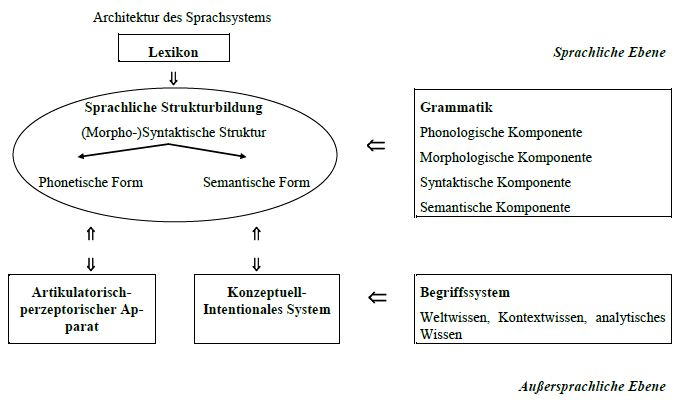
\includegraphics[scale=.3]{material/03ArchitekturSprachsystem}
%	\caption{Architektur des Sprachsystems}
%\end{figure}
%
%\end{frame}

\begin{frame}
\begin{figure}
	\centering
	
\scalebox{.72}{\begin{tikzpicture}
\node[above] at (0,0.3) {Architektur des Sprachsystems};
\node[below] at (0,0.3) [rectangle,draw]{\textbf{Lexikon}};
\node at (7.5,-0.3) {\textit{Sprachliche Ebene}};
\node at (7.5, -8) {\textit{Außersprachliche Ebene}};
\draw[->, thick] (0,-0.3)--(0,-0.8);
\draw (0,-2.5) ellipse (110pt and 45 pt);
\draw[->, thick] (0,-2.3)--(-2,-2.6);
\node[below] at (-2,-2.6) {Phonetische Form};
\draw[->, thick] (0,-2.3)--(2,-2.6);
\node[below] at (2,-2.6) {Semantische Form};
\node at (0,-1.5) {\textbf{Sprachliche Strukturbildung}};
\node at (0,-2) {(Morpho-)Syntaktische Struktur};
\draw[<->, thick] (-2,-4.3)--(-2,-5.2);
\draw[<->, thick] (2,-4.3)--(2,-5.2);
\draw[<-, thick] (4,-2.5)--(4.5,-2.5);
\draw[<-, thick] (4,-6)--(4.5,-6);
\node[below,text width=3.4 cm, align=center] (A) at (-2,-5.5) [rectangle, draw] {\textbf{Artikulatorisch-perzeptorischer Apparat}};
\node[below,text width=3.5 cm, align=center] (B) at (2,-5.5) [rectangle, draw] {\textbf{Konzeptuell-intentionales System}};
\node (C) at (7.4, -2.5) {\framebox
		{\begin{varwidth}{\linewidth}\begin{itemize}
			\item[] \textbf{Grammatik}
			\item[] Phonologische Komponente
			\item[] Morphologische Komponente
			\item[] Syntaktische Komponente
			\item[] Semantische Komponente
			\end{itemize}\end{varwidth}}
};
\node (D) at (7.3, -6.4) {\framebox
	{\begin{varwidth}{6.5cm}\begin{itemize}
		\item[] \textbf{Begriffssystem}
		\item[] Weltwissen, Kontextwissen, analytisches Wissen
		\end{itemize}\end{varwidth}}
};
\end{tikzpicture}}
	\caption{Architektur des Sprachsystems}
\end{figure}

\end{frame}


%%%%%%%%%%%%%%%%%%%%%%%%%%%%%%%%%%
%%%%%%%%%%%%%%%%%%%%%%%%%%%%%%%%%%
\subsubsection{Ziele der X-Bar-Theorie}

%\iftoggle{sectoc}{
%	\frame{
%		%\begin{multicols}{2}
%		\frametitle{~}
%		\tableofcontents[currentsubsection,subsubsectionstyle=hide]
%		%\end{multicols}
%	}
%}


%%%%%%%%%%%%%%%%%%%%%%%%%%%%%%%%%%
\begin{frame}
\frametitle{Ziele der X-Bar-Theorie}

\begin{itemize}
	\item Explikation der syntaktischen Beziehungen zwischen einem Kopf und seinen modifizierenden (\textbf{Adjunkten}), spezifizierenden (\textbf{Spezifikatoren}), und ergänzenden (\textbf{Argumenten}) Einheiten
	\item Explikation endozentrischer Konstruktionen
	\item Bis dahin wurden Sätze als exozentrische Konstruktionen behandelt!
\end{itemize}

\begin{figure}[b]
	\begin{minipage}[b]{0.05\textwidth}
	\end{minipage} 
	%
	\begin{minipage}[b]{0.50\textwidth}
	\centering
	\footnotesize{
		\begin{forest}
		sm edges,
		[S	[NP [Stefan,roof]]
			[VP [schreibt ein Buch,roof]]
		]
		\end{forest}
		}
		\caption{Satz vor X-Bar-Schema}	
  	\end{minipage}  
  	%  
	\begin{minipage}[b]{0.05\textwidth}
  	\end{minipage}
  	
\end{figure}

\end{frame}


%%%%%%%%%%%%%%%%%%%%%%%%%%%%%%%%%%
%%%%%%%%%%%%%%%%%%%%%%%%%%%%%%%%%%
\subsection{Strukturelle Annahmen}

\iftoggle{sectoc}{
	\frame{
		%\begin{multicols}{2}
		\frametitle{~}
		\tableofcontents[currentsubsection,subsubsectionstyle=hide]
		%\end{multicols}
	}
}

%%%%%%%%%%%%%%%%%%%%%%%%%%%%%%%%%%
\begin{frame}
\frametitle{X-Bar: Strukturelle Annahmen}

\citep[vgl.][]{Chomsky&Lasnik93a, Fries&MyP16a}

\begin{enumerate}
	\item[1.] Alle syntaktischen Phrasen haben \textbf{den gleichen syntaktischen Aufbau}.
\end{enumerate}


\begin{columns}

\begin{column}{.3\textwidth}
{\footnotesize	
\begin{itemize}
	\item XP: Phrase
	\item \MyPxbar{X}: Zwischenprojektion
	\item \zerobar{X}: Kopf
	\item YP: Spezifikator
	\item ZP: Komplement
\end{itemize}
}
\end{column}
%%
%%
\begin{column}{.7\textwidth}
\begin{figure}[b]
\centering
\begin{forest}
	MyP edges,
	[\alertred{XP} [\alertgreen{YP}]
	[\alertred{\MyPxbar{X}} [\alertred{\zerobar{X}}]
	[\alertgreen{ZP}]
	]
	]
\end{forest}
\caption{X-Bar-Schema}	
	
\end{figure}
\end{column}
	
\end{columns}

\end{frame}


%%%%%%%%%%%%%%%%%%%%%%%%%%%%%%%%%%
\begin{frame}
\frametitle{X-Bar: Strukturelle Annahmen}

	\begin{enumerate}
		\item[2.] Jede Phrase hat ein einziges, strukturell obligatorisches Element. 
		
		\ras \textbf{Kopf} der Phrase (Notation: \zerobar{X} oder X)
	\end{enumerate}

\begin{figure}[b]

\centering
\begin{forest}
	MyP edges,
	[XP [YP]
	[\MyPxbar{X} [\zerobar{X}, draw, HUred]
	[ZP]
	]
	]
\end{forest}
\caption{X-Bar-Schema}	
	
\end{figure}

\end{frame}


%%%%%%%%%%%%%%%%%%%%%%%%%%%%%%%%%%
\begin{frame}
\frametitle{X-Bar: Strukturelle Annahmen}

	\begin{enumerate}
		\item[3.] Zwischen Phrase und Kopf gibt es syntaktisch relevante Zwischenstufen 
		
		\ras \textbf{Zwischenprojektionen} (Notation: \MyPxbar{X} oder \ibar{X})
	\end{enumerate}


\begin{figure}[b]
\centering
\begin{forest}
MyP edges,
[XP 
	[YP]
	[\MyPxbar{X}, draw, HUred 
		[\zerobar{X}]
		[ZP]
	]
]
\end{forest}
\caption{X-Bar-Schema}	

\end{figure}

\end{frame}


%%%%%%%%%%%%%%%%%%%%%%%%%%%%%%%%%%
\begin{frame}
\frametitle{X-Bar: Strukturelle Annahmen}

	\begin{enumerate}
		\item[4.] Alle Nicht-Köpfe sind \textbf{maximale Projektionen} (bzw. Phrasen).
		
		\ras Notation: XP oder \xxbar{X} oder \iibar{X} oder \maxbar{X} oder  X$^2$
	\end{enumerate}

\begin{figure}[b]
\centering
\begin{forest}
	MyP edges,
	[XP [YP, draw, HUred]
	[\MyPxbar{X} [\zerobar{X}]
	[ZP, draw, HUred]
	]
	]
\end{forest}
\caption{X-Bar-Schema}	

\end{figure}

\end{frame}


%%%%%%%%%%%%%%%%%%%%%%%%%%%%%%%%%%
\begin{frame}
\frametitle{X-Bar: Strukturelle Annahmen}

	\begin{enumerate}
		\item[5.] Maximale Projektionen haben die gleiche Bar-Anzahl ($=2$).
		
		\ras Notation: XP oder \xxbar{X} oder \iibar{X} oder \maxbar{X} oder  X$^2$
	\end{enumerate}

\begin{figure}[b]
\centering
\begin{forest}
	MyP edges,
	[XP{$=$}X$^2$, draw, HUred
		[YP{$=$}Y$^2$, draw, HUred]
		[X$^1$ 
			[\zerobar{X}]
			[ZP{$=$}Z$^2$, draw, HUred]
		]
	]
\end{forest}
\caption{X-Bar-Schema}	

\end{figure}

\end{frame}



%%%%%%%%%%%%%%%%%%%%%%%%%%%%%%%%%%
\begin{frame}
\frametitle{X-Bar: Strukturelle Annahmen}

\begin{enumerate}
	\item[6.] Nur Nicht-Köpfe sind optional.
\end{enumerate}

\begin{columns}
	
\begin{column}{.5\textwidth}

\begin{figure}[b]
\centering
\begin{forest}
	MyP edges,
	[*XP [YP]
	[\MyPxbar{X} 
	[ZP]
	]
	]
\end{forest}
\caption{X-Bar-Schema}
\end{figure}
	
\end{column}
%%
%%
\begin{column}{.5\textwidth}

\begin{figure}[b]
	\centering
	\begin{forest}
		MyP edges,
		[XP 
		[\MyPxbar{X} [\zerobar{X}, draw, HUred]
		]
		]
	\end{forest}
	\caption{X-Bar-Schema}
\end{figure}
	
\end{column}

\end{columns}

\end{frame}


%%%%%%%%%%%%%%%%%%%%%%%%%%%%%%%%%%
%%%%%%%%%%%%%%%%%%%%%%%%%%%%%%%%%%
\subsection{Kopf}

\iftoggle{sectoc}{
	\frame{
		%\begin{multicols}{2}
		\frametitle{~}
		\tableofcontents[currentsubsection,subsubsectionstyle=hide]
		%\end{multicols}
	}
}


%%%%%%%%%%%%%%%%%%%%%%%%%%%%%%%%%%
\begin{frame}
\frametitle{Kopf}

\begin{itemize}
	\item Köpfe sind bereits aus der Morphologie bekannt.
\end{itemize}

\begin{figure}[b]
	\begin{minipage}[b]{0.05\textwidth}
	\end{minipage} 
	%
  	\begin{minipage}[b]{0.60\textwidth}
	\centering
	\small{
		\begin{forest}
		sm edges,
		[Auto\alertred{fahrer}
			[Auto] 
			[Fahrer]{\draw[<-,HUred] (.south east)--++(0em,-1.5ex)--++(+2em,0pt)
node[anchor=west,align=center]{Kopf};}
		]
		\end{forest}
		}
		\caption{Endozentrisches Kompositum}
  	\end{minipage}  
  	%              
	\begin{minipage}[b]{0.05\textwidth}
  	\end{minipage}
  	
\end{figure}

\begin{itemize}
	\item Der morphologische Kopf bestimmt die \textbf{morphosyntaktischen Eigenschaften} eines Wortes (Kasus, Numerus, Genus, Flexionsart, syntaktische Kategorie, auch semantische Aspekte, \dots ).
\end{itemize}

\end{frame}


%%%%%%%%%%%%%%%%%%%%%%%%%%%%%%%%%%
\begin{frame}
\frametitle{Kopf}

\begin{block}{}
Der Kopf einer Wortgruppe/""Konstituente/""Phrase/""Projektion ist dasjenige Element, das \textbf{die wichtigsten Eigenschaften} der Wortgruppe/""Konstituente/""Phrase/""Projektion bestimmt. 

Gleichzeitig steuert der Kopf den \textbf{Aufbau} der Phrase, d.\,h. der Kopf verlangt die Anwesenheit bestimmter anderer Elemente in seiner Phrase.

\citep[vgl.][]{Adger04a, MuellerS13f, MyP18b}
\end{block}

\pause

\begin{itemize}
	\item Was sind \gqq{die wichtigsten Eigenschaften}?
		\begin{itemize}
			\item Interpretation der Phrase
			\item Distribution der Phrase
			\item Morphosyntaktische Eigenschaften der Phrase
			\item Aufbau der Phrase	
		\end{itemize}
\end{itemize}

\end{frame}

%%%%%%%%%%%%%%%%%%%%%%%%%%%%%%%%%%
%%%%%%%%%%%%%%%%%%%%%%%%%%%%%%%%%%
\subsubsection{Interpretation}

%\iftoggle{sectoc}{
%	\frame{
%		%\begin{multicols}{2}
%		\frametitle{~}
%		\tableofcontents[currentsubsection,subsubsectionstyle=hide]
%		%\end{multicols}
%	}
%}

%%%%%%%%%%%%%%%%%%%%%%%%%%%%%%%%%%%
\begin{frame}
\frametitle{Interpretation}

\begin{itemize}
	\item Sehr intuitives (aber etwas unzuverlässiges) Kriterium, v.\,a. stark theorieabhängig
	\item Durch Konstituententests wissen wir, welche Wortfolgen \textbf{Konstituenten} sind.
\end{itemize}
\pause

\ea Peter kauft \alertred{[das erfrischende Wasser, das ich dir letztens empfohlen habe]}.

\pause

\settowidth\jamwidth{Vorfeldtest}
\ex \alertred{{[}Das erfrischende Wasser, das ich dir letztens empfohlen habe]} kauft Peter.  \jambox{ [\textbf{Vorfeldtest}]}

\pause

\ex \alertred{{[}Was]} kauft Peter? \ras \alertred{{[}Das erfrischende Wasser, das ich dir letztens empfohlen habe]} \jambox{ [\textbf{Fragetest}]}
\z

\pause
\begin{itemize}
	\item Aber welches Wort in einer Konstituente ist der \textbf{Kopf}?
\end{itemize} 

\end{frame}


%%%%%%%%%%%%%%%%%%%%%%%%%%%%%%%%%%
\begin{frame}
\frametitle{Interpretation}

\begin{itemize}
	\item Welches Element in den folgenden (markierten) Phrasen steuert die Interpretation?
\end{itemize}

\pause 
	
	\ea Peter kauft \alertred{[das erfrischende Wasser, das ich dir letztens empfohlen habe]}

\pause
	
	\ras \emph{Wasser} (Entität)

\pause
	\ex Peter wartet \alertred{[an der Ecke]}.

\pause
	\ras \emph{an} (Lokation)

\pause

	\ex Peter \alertred{[wartet an der Ecke]}.
	
 \pause

	\ras \emph{wartet} (Handlung)
	
	\z 
	
\end{frame}


%%%%%%%%%%%%%%%%%%%%%%%%%%%%%%%%%%
%%%%%%%%%%%%%%%%%%%%%%%%%%%%%%%%%%
\subsubsection{Distribution}

%\iftoggle{sectoc}{
%	\frame{
%		%\begin{multicols}{2}
%		\frametitle{~}
%		\tableofcontents[currentsubsection,subsubsectionstyle=hide]
%		%\end{multicols}
%	}
%}

%%%%%%%%%%%%%%%%%%%%%%%%%%%%%%%%%%%
\begin{frame}
\only<presentation>{\frametitle{Distribution}}

\begin{itemize}
	\item Der Kopf bestimmt, an welchen Positionen im Satz seine projizierte Phrase stehen kann:
	\begin{itemize}
		\item VPs: [\textbf{schläft}], [\textbf{kauft} den Wagen], [\textbf{schenkt} Maria die Blumen]
		\item NP: [\textbf{Peter}], [der \textbf{Wagen}], [der vermeintlich korrupte \textbf{Präsident} der FIFA]
		\item AP: [\textbf{nett}], [auf seinen Sohn \textbf{stolz}], [seiner Frau \textbf{treu}]
\end{itemize}
	\pause


\ea {S \ras NP $+$ VP}

\ea[]{Peter $+$ VP}
\ex[]{Peter $+$ [\textbf{schläft}].}
\ex[]{Peter $+$ [\textbf{kauft} den Wagen].}
\ex[]{Peter $+$ [\textbf{schenkt} Maria die Blumen].}
\ex[*]{Peter $+$ [der \textbf{Wagen}]}
\ex[*]{Peter $+$ [seiner Frau \textbf{treu}]}
\z

\z 
	
	
\end{itemize}

\end{frame}


%%%%%%%%%%%%%%%%%%%%%%%%%%%%%%%%%%%
\begin{frame}
\only<presentation>{\frametitle{Distribution}}

\begin{itemize}
	\item Der Kopf bestimmt, an welchen Positionen im Satz seine projizierte Phrase stehen kann:
	\begin{itemize}
		\item VPs: [\textbf{schläft}], [\textbf{kauft} den Wagen], [\textbf{schenkt} Maria die Blumen]
		\item NP: [\textbf{Peter}], [der \textbf{Wagen}], [der vermeintlich korrupte \textbf{Präsident} der FIFA]
		\item AP: [\textbf{nett}], [auf seinen Sohn \textbf{stolz}], [seiner Frau \textbf{treu}]
\end{itemize}
	\pause

\ea S \ras NP $+$ VP

\ea[]{NP $+$ parkt an der Ecke}
\ex[]{[\textbf{Peter}] $+$ parkt an der Ecke.}
\ex[]{[Der \textbf{Wagen}] $+$ parkt an der Ecke.}
\ex[]{[Der vermeintlich korrupte \textbf{Präsident} der FIFA] $+$ parkt an der Ecke.}
\ex[*]{[\textbf{Schläft}] $+$ parkt an der Ecke.}
\ex[*]{[\textbf{Nett}] $+$ parkt an der Ecke.}
\z

\z	
	
\end{itemize}

\end{frame}


%%%%%%%%%%%%%%%%%%%%%%%%%%%%%%%%%%%
\begin{frame}
\only<presentation>{\frametitle{Distribution}}

\begin{itemize}
	\item Der Kopf bestimmt, an welchen Positionen im Satz seine projizierte Phrase stehen kann:
	\begin{itemize}
		\item VPs: [\textbf{schläft}], [\textbf{kauft} den Wagen], [\textbf{schenkt} Maria die Blumen]
		\item NP: [\textbf{Peter}], [der \textbf{Wagen}], [der vermeintlich korrupte \textbf{Präsident} der FIFA]
		\item AP: [\textbf{nett}], [auf seinen Sohn \textbf{stolz}], [seiner Frau \textbf{treu}]
\end{itemize}
	\pause

\ea NP \ras Det $+$ (AP) $+$ N

\ea[]{Der $+$ AP $+$ N}
\ex[]{Der $+$ [\textbf{nette}] $+$ Onkel}
\ex[]{Der $+$ [auf seinen Sohn \textbf{stolze}] $+$ Onkel}
\ex[]{Der $+$ [seiner Frau \textbf{treue}] $+$ Onkel}
\ex[*]{Der $+$ [\textbf{schläft}] $+$ Onkel}
\ex[*]{Der $+$ [der \textbf{Wagen}] $+$ Onkel}
\z
	
\z	

\end{itemize}

\end{frame}

%%%%%%%%%%%%%%%%%%%%%%%%%%%%%%%%%%
%%%%%%%%%%%%%%%%%%%%%%%%%%%%%%%%%%
\subsubsection{Morphosyntaktische Eigenschaften}

%\iftoggle{sectoc}{
%	\frame{
%		%\begin{multicols}{2}
%		\frametitle{~}
%		\tableofcontents[currentsubsection,subsubsectionstyle=hide]
%		%\end{multicols}
%	}
%}

%%%%%%%%%%%%%%%%%%%%%%%%%%%%%%%%%%%
\begin{frame}
\only<presentation>{\frametitle{Morphosyntaktische Eigenschaften}}

\begin{itemize}
	\item \textbf{Kategorielle Zugehörigkeit} (Wortart \ras Phrasentyp)\\
	\ras Wenn der Kopf ein \textbf{Nomen} ist, ist die gesamte Phrase eine \textbf{NP}.\\
	\ras Wenn der Kopf ein \textbf{Verb} ist, ist die gesamte Phrase eine \textbf{VP}.
\end{itemize}

\begin{figure}[b]
%	\begin{minipage}[b]{0.05\textwidth}
%	\end{minipage} 
	%
	\begin{minipage}[b]{0.40\textwidth}
	\centering
	\scalebox{.68}{
	\hfill	\begin{forest}
		MyP edges,
		[VP [NP [Peter,roof]]
			[\MyPxbar{V} [NP [den Patienten,roof]]
				[V [behandelt]]		{\draw[<-,HUred] (.south east)--++(0em,-1.5ex)--++(+2em,0pt)
node[anchor=west,align=center]{Kopf};}
			]
		]
		\end{forest}
		}
		\caption{VP}	
  	\end{minipage}  
  	%  
  	\pause            
	\begin{minipage}[b]{0.05\textwidth}
		\hfill
  	\end{minipage}
  	%         
  	\begin{minipage}[b]{0.40\textwidth}
	\centering
	\scalebox{.68}{
	\hfill	\begin{forest}
		MyP edges,
		[NP [Det [Peters]]
			[\MyPxbar{N} [AP [sanfte,roof]]
				[\MyPxbar{N} [N [Behandlung]]{\draw[<-,HUred] (.south west)--++(0em,-1.5ex)--++(-2em,0pt)
node[anchor=east,align=center]{Kopf};}
					[NP [des Patienten,roof]]]]
		]
		\end{forest}
		}
		\caption{NP}
  	\end{minipage}  
  	%              
%	\begin{minipage}[b]{0.05\textwidth}
%  	\end{minipage}
  	
\end{figure}


\end{frame}


%%%%%%%%%%%%%%%%%%%%%%%%%%%%%%%%%%
\begin{frame}
\only<presentation>{\frametitle{Morphosyntaktische Eigenschaften}}

\begin{itemize}
	\item Der Kopf \textbf{projiziert} seine Merkmale auf die gesamte Phrase. 
\end{itemize}

\begin{tabular}{ll}
\textsc{Wortart} & \textsc{Merkmale}\\
\hline
\textbf{Verb}		& Wortart, Numerus-tragend, Person-tragend, Kasus-\\
					& determinierend, Verbform (Finitheitsmerkmale) \\
\hline
\textbf{Nomen}		& Wortart, Kasus-tragend, (Person), Numerus-tragend,\\
					& Genus-tragend, Genitiv-determinierend\\
\hline
\textbf{Adjektiv}	& Wortart, Kasus-tragend, Genus-tragend, Numerus-\\ 
					& tragend, Flexionsklasse, Kasus-determinierend\\
\hline
\textbf{Präposition}& Wortart, nicht-Kasus-tragend, nicht-Numerus-\\
					& tragend, nicht-Genus-tragend, Kasus-\\
					& determinierend\\					
\end{tabular}
\end{frame}


%%%%%%%%%%%%%%%%%%%%%%%%%%%%%%%%%%
%%%%%%%%%%%%%%%%%%%%%%%%%%%%%%%%%%
\subsubsection{Phrasenaufbau: Argumentstruktur}

%\iftoggle{sectoc}{
%	\frame{
%		%\begin{multicols}{2}
%		\frametitle{~}
%		\tableofcontents[currentsubsection,subsubsectionstyle=hide]
%		%\end{multicols}
%	}
%}

%%%%%%%%%%%%%%%%%%%%%%%%%%%%%%%%%%
\begin{frame}
\frametitle{Phrasenaufbau: Argumentstruktur}

\begin{itemize}
	\item Auch: Valenz, Subkategorisierung
	\item[]
	\item Es wird angenommen, dass Köpfe (lexikalische Einheiten) \ua mit ihrer Argumentstruktur im \textbf{mentalen Lexikon} gespeichert sind.
	\item[]
	\item Köpfe werden aus dem Lexikon genommen und in die \textbf{syntaktische Komponente} eingefügt, wo ihre Argumentstruktur verschiedene Ebenen im X-Bar-Schema projiziert.
\end{itemize}

\end{frame}


%%%%%%%%%%%%%%%%%%%%%%%%%%%%%%%%%%
\begin{frame}
\frametitle{Phrasenaufbau: Argumentstruktur}

\begin{block}{Argumente und Modifikatoren}
Argumente sind die von einem Kopf (Nomen, Verb, Präposition, \dots ) verlangten Einheiten, um eine wohlgeformte Phrase zu bilden. Der Kopf bestimmt dabei die \textbf{Anzahl}, die \textbf{Form} (\zB Kasus) und die \textbf{Art} (\zB Theta-Rolle) seiner Argumente. Nicht-Argumente in einer Struktur werden \textbf{Modifikatoren} genannt. Sie werden nicht verlangt, sondern können frei hinzugefügt werden und \textbf{modifizieren} die Aussage. 
\end{block}

\end{frame}


%%%%%%%%%%%%%%%%%%%%%%%%%%%%%%%%%%%
\begin{frame}
\frametitle{Phrasenaufbau: Argumentstruktur}

\begin{itemize}
	\item Der Kopf bestimmt, \textbf{welche und wieviele} Argumente \textbf{notwendig} sind, um eine wohlgeformte Phrase zu bilden.

\settowidth\jamwidth{(3 Argumente)}
\eal 
\ex {[Clara] schläft.} \jambox{(1 Argument)}
\ex {[Clara] küsst [Maria].} \jambox{(2 Argumente)}
\ex {[Maria] schenkt [Clara] [die Blumen].} \jambox{(3 Argumente)}
\zl

\pause

\eal
\ex[*]{[Clara] schläft [Maria].}
\ex[*]{[Maria] küsst [Clara] [die Blumen].}
\ex[*]{schenkt.}
\zl


\end{itemize}
\end{frame}


%%%%%%%%%%%%%%%%%%%%%%%%%%%%%%%%%%%
\begin{frame}
\only<presentation>{\frametitle{Phrasenaufbau: Argumentstruktur}}

\begin{itemize}
	\item Der Kopf bestimmt \textbf{die Form} seiner Argumente (\zB durch \textbf{Kasusrektion}).
\end{itemize}

\eal 
\ex {[Der Mann]$_{\textsc{nom}}$ schläft.}
\ex {[Der Mann]$_{\textsc{nom}}$ küsst [den Elefanten]$_{\textsc{akk}}$.}
\ex {[Der Mann]$_{\textsc{nom}}$ schenkt [dem Jungen]$_{\textsc{dat}}$ [den Elefanten]$_{\textsc{akk}}$.}
\ex {[Der Mann]$_{\textsc{nom}}$ gedenkt [des Opfers]$_{\textsc{gen}}$.}
\ex {[Der Mann]$_{\textsc{nom}}$ hilft [dem Opfer]$_{\textsc{dat}}$.}
\ex {[Der Mann]$_{\textsc{nom}}$ wartet [auf den Jungen]$_{auf}$.}
\zl

\pause

\eal
\ex[*]{[Der Mann]$_{\textsc{nom}}$ gedenkt [dem Opfer]$_{\textsc{dat}}$.}
\ex[*]{[Der Mann]$_{\textsc{nom}}$ hilft [des Opfers]$_{\textsc{gen}}$.}
\ex[*]{[Der Mann]$_{\textsc{nom}}$ wartet [den Jungen]$_{\textsc{akk}}$.}
\zl

\end{frame}


%%%%%%%%%%%%%%%%%%%%%%%%%%%%%%%%%%%
\begin{frame}
\only<presentation>{\frametitle{Phrasenaufbau: Argumentstruktur}}

\begin{itemize}
	\item Der Kopf bestimmt \textbf{die Form} seiner Argumente (\zB durch \textbf{Finitheitsrektion}).
\end{itemize}

\ea \textbf{Modalverb} verlangt Infinitiv\\
\dots dass er es \alertred{kaufen$_{\textsc{inf}}$ will}
\pause
\ex \textbf{\emph{haben}-Hilfsverb} verlangt Partizip II\\
\dots dass er es \alertred{gekauft$_{\textsc{part}}$ hat}
\pause
\ex \textbf{Modalverb} verlangt Infinitiv\\
\dots dass er es \alertred{[gekauft haben]$_{\textsc{inf}}$ will}
\pause
\ex \textbf{Modalverb} verlangt Infinitiv\\
\dots dass er es \alertred{[gekauft haben wollen]$_{\textsc{inf}}$ muss}
\pause
\ex \textbf{\emph{haben}-Hilfsverb} verlangt Partizip II\\
\dots dass er es \alertred{[gekauft haben wollen müssen/gemusst]$_{\textsc{inf}}$ hat}
\z

\end{frame}


%%%%%%%%%%%%%%%%%%%%%%%%%%%%%%%%%%%
\begin{frame}
\only<presentation>{\frametitle{Phrasenaufbau: Argumentstruktur}}

\begin{itemize}
	\item Der Kopf bestimmt \textbf{die Art}, wie seine Argumente interpretiert werden (Theta-Rollen, $\theta$-Rollen).

\eal 
\ex {[Der Elefant]$_{\textsc{agens}}$ tötet [den Mann]$_{\textsc{patiens}}$.}
\ex {[Der Elefant]$_{\textsc{thema}}$ interessierte [den Mann]$_{\textsc{experiencer}}$.}
\zl

\eal
\ex {[Peters]$_{\textsc{agens}}$ Behandlung [des Mannes]$_{\textsc{patiens}}$}
\ex {[Peters]$_{\textsc{patiens}}$ Ermordung}
\zl


	\item Einige Verben (\zB \MyPobj{regnen, schneien}) vergeben ihrem Subjekt keine Theta-Rolle. Sie sind semantisch gesehen \textbf{0-wertig}.

\end{itemize}

\end{frame}


%%%%%%%%%%%%%%%%%%%%%%%%%%%%%%%%%%
%%%%%%%%%%%%%%%%%%%%%%%%%%%%%%%%%%
\subsection{Theta-Rollen}

\iftoggle{sectoc}{
	\frame{
		%\begin{multicols}{2}
		\frametitle{~}
		\tableofcontents[currentsubsection,subsubsectionstyle=hide]
		%\end{multicols}
	}
}

%%%%%%%%%%%%%%%%%%%%%%%%%%%%%%%%%%
\begin{frame}
\frametitle{Theta-Rollen}

\begin{itemize}
	\item Auch: thematische/""semantische Rollen, Theta-Rollen, $\theta$-Rollen
\medskip	
	\item[]
	\item Semantische Rolle, die ein Argument von seinem Kopf erhält
\medskip	
	\item[]
	\item Anzahl und Definition der Theta-Rollen: theorieabhängig

	\begin{itemize}
		\item \textbf{AGENS:} jemand, der die Handlung, die durch das Prädikat bezeichnet wird, willentlich anstößt/""ausführt.
\medskip		
		\item[]
		\item \textbf{THEMA/""PATIENS:} jemand oder etwas, der oder das durch die vom Prädikat bezeichnete Handlung betroffen wird
\medskip		
		\item[]
		\item \textbf{EXPERIENCER:} jemand, der durch die (in der) vom Prädikat bezeichneten Handlung etwas psychisch oder physisch empfindet

	\end{itemize}

\end{itemize}

\end{frame}


%%%%%%%%%%%%%%%%%%%%%%%%%%%%%%%%%%
\begin{frame}
\frametitle{Theta-Rollen}

\begin{itemize}
	\item Anzahl und Definition der Theta-Rollen \ras theorieabhängig
	
	\begin{itemize}

		\item \textbf{ZIEL (GOAL):} die Entität, auf die die vom Prädikat ausgedrückte Handlung gerichtet ist
\medskip
		\item[]
		\item \textbf{QUELLE (SOURCE):} die Entität, von der die vom Prädikat ausgedrückte Handlung ausgeht
\medskip
		\item[]
		\item \textbf{ORT (LOCATION):} der Ort, an dem die vom Prädikat ausgedrückte Handlung stattfindet
\medskip
		\item[]
		\item \textbf{ZEIT (TIME):} die Zeit(spanne), an der die vom Prädikat ausgedrückte Handlung stattfindet
\medskip
		\item[]
		\item \textbf{POSSESSOR:} Entität, die ein Objekt besitzt		
	\end{itemize}

\end{itemize}

\end{frame}


%%%%%%%%%%%%%%%%%%%%%%%%%%%%%%%%%%
%%%%%%%%%%%%%%%%%%%%%%%%%%%%%%%%%%
\subsection{Subkategorisierungsrahmen}

\iftoggle{sectoc}{
	\frame{
		%\begin{multicols}{2}
		\frametitle{~}
		\tableofcontents[currentsubsection,subsubsectionstyle=hide]
		%\end{multicols}
	}
}

%%%%%%%%%%%%%%%%%%%%%%%%%%%%%%%%%%
\begin{frame}
\frametitle{Subkategorisierungsrahmen}

\begin{itemize}
	\item Information im Subkategorisierungsrahmen einer Kategorie:
	\item[]
	\begin{enumerate}
		\item \textbf{Anzahl} der benötigten Argumente (syntaktische Information),
		\item[]
\medskip		
		\item ihre \textbf{syntaktische Kategorie} (DP, PP, CP, \dots )\\
		(syntaktische Information: c-selektionales Merkmal oder Subkategorisierungseigenschaft),
\medskip		
		\item[]
		\item ihre \textbf{morphosyntaktische Realisierung} (\zB Kasus) (morphologische Information),
\medskip		
		\item[]
		\item ihre \textbf{$\theta$-Rolle} (semantische Information),
\medskip		
		\item[]
		\item \textbf{weitere semantische Eigenschaften}, \zB das Objekt vom Verb \MyPobj{trinken} muss \gqq{flüssig} sein (semantische Information: s-selektionales Merkmal oder 	Selektionsbeschränkung).
	\end{enumerate}
	
\end{itemize}

\end{frame}


%%%%%%%%%%%%%%%%%%%%%%%%%%%%%%%%%%
\begin{frame}
\frametitle{Subkategorisierungsrahmen}

\begin{itemize}

	\item Die Information der Argumentstruktur im Subkategorisierungsrahmen:
	
	\ea lesen: DP$_{\textsc{nom,ag}}$ (DP)$_{\textsc{akk,th}}$ $\underline{\qquad}$
	\z
	
	\item[] \textbf{$=$} \MyPobj{lesen} ist subkategorisiert für zwei Argumente, die beide syntaktisch NPn/DPn sind. Eine der NPn/DPn ist obligatorisch, wird im Nominativ realisiert und trägt die $\theta$-Rolle Agens, z.B. \MyPobj{Uta} in \MyPobj{Uta liest ein Buch}. Die andere NP/DP ist fakultativ, wird im Akkusativ realisiert und trägt die $\theta$-Rolle Thema (\zB \MyPobj{ein Buch} in \MyPobj{Uta liest ein Buch}).

	\ea schenken: DP$_{\textsc{nom,ag}}$ DP$_{\textsc{dat,ziel}}$  DP$_{\textsc{akk,th}}$ $\underline{\qquad}$ 
	\z
		
\end{itemize}

\end{frame}


%%%%%%%%%%%%%%%%%%%%%%%%%%%%%%%%%%
%%%%%%%%%%%%%%%%%%%%%%%%%%%%%%%%%%
\subsection{Modifikatoren (vs. Argumente)}

\iftoggle{sectoc}{
	\frame{
		%\begin{multicols}{2}
		\frametitle{~}
		\tableofcontents[currentsubsection,subsubsectionstyle=hide]
		%\end{multicols}
	}
}

%%%%%%%%%%%%%%%%%%%%%%%%%%%%%%%%%%
\begin{frame}

\textbf{Modifikatoren} sind vom Kopf weitgehend unabhängig in Bezug auf\dots

\begin{itemize}
	\item \textbf{Anzahl}

\eal 
\ex Maria schläft \alertred{[heute] [im Zimmer] [unruhig]}.
\ex Maria küsst Clara \alertred{[heute] [im Zimmer] [unruhig]}.
\ex Maria schenkt Clara die Blumen \alertred{[heute] [im Zimmer] [unruhig]}.
\zl

	\begin{itemize}
		\item Modifikatoren sind \textbf{immer fakultativ}!
		\item Argumente können \textbf{obligatorisch} oder \textbf{fakultativ} sein (sie werden dann \gqq{mitverstanden}: existentielle Interpretation).
		
		\eal 
		\ex Maria schläft \alertred{[heute] [im Zimmer]}.
		\ex Maria schläft \alertred{[im Zimmer]}. 
		\zl
		
		\eal 
		\ex Clara isst \alertred{[eine Schokolade]}.
		\ex Clara isst. 
		\zl
		
	\end{itemize}

\end{itemize}

\end{frame}


%%%%%%%%%%%%%%%%%%%%%%%%%%%%%%%%%%
\begin{frame}

\textbf{Modifikatoren} (syntaktisch: Adjunkte) sind vom Kopf weitgehend unabhängig in Bezug auf\dots

\begin{itemize}
	
	\item \textbf{Form}
\eal
\ex Maria schläft \alertred{[heute]$_{AdvP}$ [im Zimmer]$_{PP}$, [obwohl die Heizung nicht funktioniert]$_{CP}$}.
\ex Maria küsst Clara \alertred{[heute]$_{AdvP}$ [im Zimmer]$_{PP}$, [obwohl die Heizung nicht funktioniert]$_{CP}$}.
\ex Maria schenkt Clara die Blumen \alertred{[heute]$_{AdvP}$ [im Zimmer]$_{PP}$, [obwohl die Heizung nicht funktioniert]$_{CP}$}.
\zl

\end{itemize}

\end{frame}


%%%%%%%%%%%%%%%%%%%%%%%%%%%%%%%%%%
\begin{frame}

\textbf{Modifikatoren} (syntaktisch: Adjunkte) sind vom Kopf weitgehend unabhängig in Bezug auf\dots

\begin{itemize}
	\item \textbf{Art}

\eal 
\ex Der Ingenieur sprengte \alertred{[die Brücke]$_{\textsc{pat}}$}. 
\ex Der Ingenieur sah \alertred{[die Brücke]$_{\textsc{th}}$}. 
\ex Der Ingenieur verließ \alertred{[die Brücke]$_{\textsc{quelle}}$}.
\zl

	\begin{itemize}
		\item Modifikatoren der gleichen Art sind \textbf{iterierbar}!
		\item Argumente der gleichen Art sind \textbf{nicht iterierbar}!
		
		\eal 
		\ex[]{Maria schläft \alertred{[heute]$_{\textsc{zeit}}$ [am frühen Morgen]$_{\textsc{zeit}}$}.}
		\ex[*]{Peter isst \alertred{[eine Schokolade]$_{\textsc{th}}$ [einen Kuchen]$_{\textsc{th}}$}.}
		\zl

		
	\end{itemize}

\end{itemize}

\end{frame}


%%%%%%%%%%%%%%%%%%%%%%%%%%%%%%%%%%
%%%%%%%%%%%%%%%%%%%%%%%%%%%%%%%%%%
\subsection{Hausaufgabe}


%%%%%%%%%%%%%%%%%%%%%%%%%%%%%%%%%%%	

	
\begin{frame}
\frametitle{Hausaufgabe}

\begin{itemize}

	\item Bestimmen Sie den Kopf der folgenden \textbf{markierten} Phrasen und begründen Sie Ihre Entscheidung:
	
	\ea\label{ex:KopfSchueler} Es geht um [\textbf{wirklich von dieser Sache überzeugte und engagierte junge Schüler, die sich dennoch über das übliche und akzeptable Ausmaß hinaus daneben benommen haben}].
	\z
	
	\ea Wir warteten auf [\textbf{den von sich sehr überzeugten Redner}].
	\z 
	
\end{itemize}

\end{frame}

%%%%%%%%%%%%%%%%%%%%%%%%%%%%%%%%%%%	

	
\begin{frame}
\frametitle{Hausaufgabe}

\begin{itemize}

	\item Geben Sie für die folgenden Wörter den Subkategorisierungsrahmen (in dem besprochenen Format) und ein(en) Beispiel(satz), der den von Ihnen angegebenen Subkategorisierungsrahmen illustriert, an:
	
	\ea übergeben
	\ex stolz
	\ex donnern
	\ex glauben
	\ex Frage
	\ex erschrecken
	\ex bemalen
	\z 
	
%	wissen, regnen, scheinen, mit, ängstigen, fürchten, Banane, Tatsache, warten, Angst, wohnen, bewohnen, auf, malen, krank, bemalen, fragen

\end{itemize}

\end{frame}

%%%%%%%%%%%%%%%%%%%%%%%%%%%%%%%%%%%	

	
\begin{frame}
\frametitle{Hausaufgabe}

\begin{itemize}
	
	\item Bestimmen Sie in den folgenden Sätzen, welche Phrasen Argumente und welche Modifikatoren des Verbs sind, und begründen Sie Ihre Entscheidung.

\end{itemize}

\ea Maria bearbeitete die Folien mit sehr viel Kreativität.

\ex Maria arbeitete an den Folien den ganzen Tag.

\ex Peter wirkte auf seinen Sohn stolz.
\z 

\end{frame}

%%%%%%%%%%%%%%%%%%%%%%%%%%%%%%%%%%%	

\iftoggle{ha-loesung}{

\begin{frame}
\frametitle{Hausaufgabe (Lösung)} 

\begin{itemize}
	\item Bestimmen Sie den Kopf der folgenden \textbf{markierten} Phrasen und begründen Sie Ihre Entscheidung:
\end{itemize}
	
	\ea Es geht um [\textbf{wirklich von dieser Sache überzeugte und engagierte junge Schüler, die sich dennoch über das übliche und akzeptable Ausmaß hinaus daneben benommen haben}].
	\z

\pause 

	
\begin{itemize}
	\item \alertred{Kopf: Schüler (vorläufig)}
	\item \alertred{Interpretation: Es geht um \emph{Schüler}}
	\item \alertred{Distribution: Innerhalb einer PP wird eine (DP/)NP selegiert. Der Kopf dieser NP ist das Nomen.}
	\item \alertred{Phrasenaufbau: Alle anderen Modifikatoren beziehen sich auf das Nomen. }
\end{itemize}

	
\end{frame}


\begin{frame}
\frametitle{Hausaufgabe (Lösung)} 

\begin{itemize}
	\item Bestimmen Sie den Kopf der folgenden Phrase und begründen Sie Ihre Entscheidung:
\end{itemize}

\ea Wir warteten auf [\textbf{den von sich sehr überzeugten Redner}].
\z 

\pause 

\begin{itemize}
	\item \alertred{Kopf: Redner (vorläufig)}
	\item \alertred{Interpretation: Es geht um \emph{Redner}}
	\item \alertred{Distribution: Innerhalb einer PP wird eine (DP/)NP selegiert. Der Kopf dieser NP ist das Nomen.}
	\item \alertred{Phrasenaufbau: Alle anderen Modifikatoren beziehen sich auf das Nomen.}
\end{itemize}
	
	
\end{frame}


\begin{frame}
\frametitle{Hausaufgabe (Lösung)} 

\begin{itemize}
	
	\item Geben Sie für die folgenden Wörter den Subkategorisierungsrahmen (in dem besprochenen Format) und ein(en) Beispiel(satz), der den von Ihnen angegebenen Subkategorisierungsrahmen illustriert, an:
	
	\ea übergeben: \pause \alertred{DP$_{\textsc{nom,quelle}}$ (DP$_{\textsc{dat,ziel}}$) DP$_{\textsc{akk,th}}$ $\underline{\qquad}$ [Lesart 1]}
	
	\alertred{(dass) ich Peter die Briefe \emph{übergebe}}
	\pause 
	
	\ex stolz: \pause \alertred{PP$_{auf+\textsc{akk,th}}$ $\underline{\qquad}$ (DP$_{\textsc{exp}}$)}
	
	\alertred{die auf ihre Tochter \emph{stolze} Mutter}
	\pause 
	
	\ex donnern: \pause \alertred{DP$_{(es),\textsc{nom}}$ $\underline{\qquad}$}
	
	\alertred{(dass) es \emph{donnert}}
	\pause
	\z 
	
	%	wissen, regnen, scheinen, mit, ängstigen, fürchten, Banane, Tatsache, warten, Angst, wohnen, bewohnen, auf, malen, krank, bemalen, fragen
	
\end{itemize}

\end{frame}


\begin{frame}
\frametitle{Hausaufgabe (Lösung)} 

\begin{itemize}

\item Geben Sie für die folgenden Wörter den Subkategorisierungsrahmen (in dem besprochenen Format) und ein(en) Beispiel(satz), der den von Ihnen angegebenen Subkategorisierungsrahmen illustriert, an:

\ea Frage: \pause \alertred{DP$_{\textsc{gen,ag}}$ $\underline{\qquad}$ PP$_{nach+\textsc{dat,th}}$}

\alertred{die Frage nach dem Schatz}
\pause 

\ex erschrecken: \pause \alertred{DP$_{\textsc{nom,causer}}$ DP$_{\textsc{akk,exp}}$ $\underline{\qquad}$ [Lesart 1]}

\alertred{(dass) Maria Peter erschreckt}
\pause 

\ex bemalen: \pause \alertred{DP$_{\textsc{nom,ag}}$ DP$_{\textsc{akk,pat/th}}$ $\underline{\qquad}$}

\alertred{(dass) ich die Wand bemale}
\z 

%	wissen, regnen, scheinen, mit, ängstigen, fürchten, Banane, Tatsache, warten, Angst, wohnen, bewohnen, auf, malen, krank, bemalen, fragen

\end{itemize}

\end{frame}

\begin{frame}
\frametitle{Hausaufgabe (Lösung)} 

\begin{itemize}
	
	\item Bestimmen Sie in den folgenden Sätzen, welche Phrasen Argumente und welche Modifikatoren des Verbs sind, und begründen Sie Ihre Entscheidung.
	
\end{itemize}

\ea Maria bearbeitete die Folien mit sehr viel Kreativität.

\pause 
\alertred{Arg.: Maria, die Folien}

\alertred{Mod.: mit sehr viel Kreatitvität}

\alertred{Begründung: \dots }

\pause 


\ex Maria arbeitete an den Folien den ganzen Tag.

\pause 
\alertred{Arg.: Maria, an den Folien}

\alertred{Mod.: den ganzen Tag}

\alertred{Begründung: \dots }

\z 

\end{frame}


\begin{frame}
\frametitle{Hausaufgabe (Lösung)} 

\begin{itemize}

\item Bestimmen Sie in den folgenden Sätzen, welche Phrasen Argumente und welche Modifikatoren des Verbs sind, und begründen Sie Ihre Entscheidung.

\end{itemize}

\ea Peter wirkte auf seinen Sohn stolz.

\pause 
\alertred{Arg.: Peter, auf seinen Sohn stolz}

\alertred{Mod.: $\emptyset$}

\alertred{Begründung: \dots }

\pause 


\ex Peter wirkte auf seinen Sohn stolz.

\pause 
\alertred{Arg.: Peter, auf seinen Sohn, stolz}

\alertred{Mod.: $\emptyset$}

\alertred{Begründung: \dots }
\z 


\end{frame}
}

%%%%%%%%%%%%%%%%%%%%%%%%%%%%%%%%%%%	
